\documentclass[10pt,twocolumn]{article}
\usepackage{graphicx}
\usepackage[margin=0.5in]{geometry}
\usepackage[cmex10]{amsmath}
\usepackage{array}
\usepackage{booktabs}
\usepackage{mathtools}
\title{\textbf{Optimization Assignment - 1}}
\author{Thoutu Rahul Raj}
\date{September 2022}


\providecommand{\norm}[1]{\lVert#1\rVert}
\providecommand{\abs}[1]{\vert#1\vert}
\let\vec\mathbf
\newcommand{\myvec}[1]{\ensuremath{\begin{pmatrix}#1\end{pmatrix}}}
\newcommand{\mydet}[1]{\ensuremath{\begin{vmatrix}#1\end{vmatrix}}}
\providecommand{\brak}[1]{\ensuremath{\left(#1\right)}}
\providecommand{\lbrak}[1]{\ensuremath{\left(#1\right.}}
\providecommand{\rbrak}[1]{\ensuremath{\left.#1\right)}}
\providecommand{\sbrak}[1]{\ensuremath{{}\left[#1\right]}}

\begin{document}

\maketitle
\paragraph{\textit{Problem Statement} - Find the maximum isosceles triangle inscribable in a given ellipse,i.e,find the maximum value of xy,having given\\
\large{$ \frac{x^2}{a^2}$+$\frac{y^2}{b^2}$=1.}\\
} 

\section{Solution}
\begin{flushleft}
Given function is,\\
\end{flushleft}
\begin{equation}
   f(x) = absin\theta(1-cos\theta)\\
\end{equation}
\subsection{Calculation using normal differentiation}
\begin{flushleft}
Differentiating (1) yields,
\end{flushleft}
\begin{align}
\nabla f(x) = ab(cos\theta-cos2\theta)
\end{align}

\noindent Calculating the critical points:
$ \nabla f(x) = 0 $

\begin{equation}
\implies \cos{\theta} = 0 
\end{equation}
\begin{equation}
\implies cos2\theta = 0
\end{equation}
Therefore, the critical points are 

\begin{equation}
{\pi}{n},\quad\frac{\pi}{2}+{\pi}n
\end{equation}

\textbf{1.1.1 Finding absolute maximum} 
Since given interval is $\quad x \in [0,n\pi]$ 

\begin{flushleft}
f attains its maximum value on the interval [0,2] at x=1.
\end{flushleft}
\center
$\implies \nabla f(1) =0$\endcenter
\center
$\implies a=1.999$\endcenter
\begin{flushleft}
\subsection{Calculation of Maxima using gradient ascent algorithm}
\end{flushleft}
\begin{flushleft}
Maxima of the above equation (1), can be calculated from the following expression,\\
\end{flushleft}
    \begin{equation}
        x_{n+1}= x_n + \alpha \nabla f(x_n)
    \end{equation}
    \begin{flushleft}
\subsection{Calculation of Maxima using gradient ascent algorithm}
\end{flushleft}
\begin{align}
	f(x) = absin\theta(1-cos\theta)\\
    f'(x) = abcos\theta-cos^2\theta+sin^2\theta
	\end{align}
we have to attain the maximum value of area of rectangle. This can be seen in Figure.Using gradient ascent method we can find its maxima.
\begin{equation}
        x_{n+1} = x_n + \alpha \nabla f(x_n) 
\end{equation}
%\begin{equation}
%	x_{n-1} = x_n - \alpha \nabla f(x_n)  
%\end{equation}
\vspace{1mm}
\begin{equation}
\implies x_{n+1}=x_n+\alpha(abcos\theta-cos^2\theta+sin^2\theta))
\end{equation}

Taking $x_0=0.5,\alpha=0.001$ and precision = 0.00000001, values obtained using python are:
    \begin{align}
        \boxed{\text{Maxima} = 1.9999}\\     
        \boxed{\text{Maxima Point} = 0.7853}
    \end{align}
\endcenter
\section{Conclusion}
\begin{flushleft}
1. At first, the given function has been differentiated and it is solved by setting f'(x) equal to zero. By using x values, f(x) values are calculated.\\
\vspace{0.25cm}
2. Later, the given function f(x) is solved by gradient ascent algorithm to find maxima and the point at which f(x) is maximum.\\
\vspace{0.25cm}
3. Then, the given function f(x) is solved by gradient descent algorithm to find minima and the point at which f(x) is is minimum.\\
\vspace{0.25cm}
\end{flushleft}
 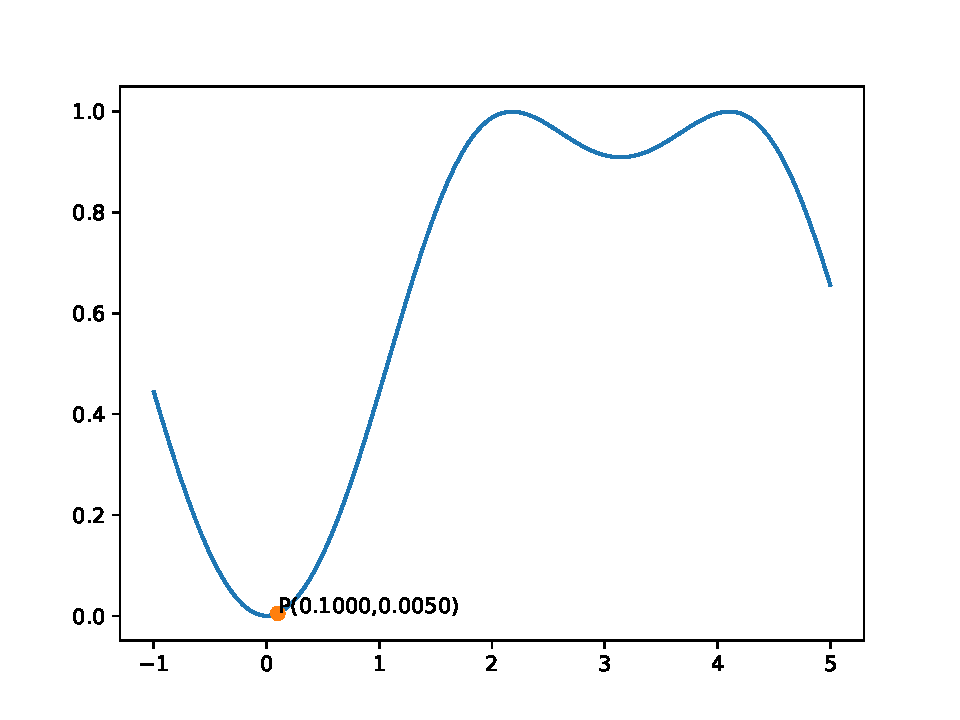
\includegraphics[scale=0.6]{opt2.pdf} 
\endcenter
\end{document}